% This is LLNCS.DOC the documentation file of
% the LaTeX2e class from Springer-Verlag
% for Lecture Notes in Computer Science, version 2.4


\documentclass{llncs}
\usepackage{llncsdoc}
%\usepackage{listings}
\usepackage{graphicx}
%\usepackage{amsmath,amsfonts,amsthm}
%\usepackage[none]{hyphenat}
%\usepackage{sectsty} % Allows customizing section commands
%\allsectionsfont{\centering \normalfont\scshape} % Make all sections centered, the default font and small caps
%\setcounter{secnumdepth}{3}
%
\begin{document}
\markboth{Proyecto Final de SRI
}{ Proyecto Final de SRI}
\thispagestyle{empty}
\begin{flushleft}
\LARGE\bfseries Carrera de Ciencia de la Computaci\'on\\
Universidad de la Habana\\[2cm]
\end{flushleft}
\rule{\textwidth}{1pt}
\vspace{2pt}
\begin{flushright}
\Huge
\begin{tabular}{@{}l}
Proyecto Final de\\
Sistemas de Recuperaci\'on de\\
Informaci\'on\\
{\Large Versi\'on 1.0}
\end{tabular}
\end{flushright}
\rule{\textwidth}{1pt}
\vfill
%\begin{flushleft}
%\large\itshape
%\begin{tabular}{@{}l}
%{\Large\upshape\bfseries Springer}\\[8pt]
%Berlin\enspace Heidelberg\enspace New\kern0.1em York\\[5pt]
%Barcelona\enspace Budapest\enspace Hong\kern0.2em Kong\\[5pt]
%London\enspace Milan\enspace Paris\enspace\\[5pt]
%Santa\kern0.2em Clara\enspace Singapore\enspace Tokyo
%\end{tabular}
%\end{flushleft}

\begin{flushleft}
\begin{tabular}{l@{\quad}l@{\hspace{3mm}}l@{\qquad}l}
$\bullet$&\multicolumn{3}{@{}l}{\bfseries Alejandro Escobar Giraudy C312}\\[1mm]
$\bullet$&\multicolumn{3}{@{}l}{\bfseries Airelys Collazo Perez C312}\\[1mm]
\end{tabular}
\end{flushleft}


%
\newpage
\tableofcontents
\newpage

%
\section{Abstracto}
%

Hoy vivimos en una era tecnol\'ogica, donde la mayor\'ia de la informaci\'on y de los documentos son digitales y se encuentran a nuestro alcance; pero, c\'omo encontrar un documento espec\'ifico entre tanta informaci\'on.
\\\\
Cada d\'ia en alg\'un lugar surge nueva informaci\'on, con el decursar del tiempo esa informaci\'on crece y crece, cuando alguien va a consultar un documento se le hace muy d\'ificil encontrarlo; imaginemos qu\'e tan dif\'icil es encontrar un art\'iculo entre millones y millones que est\'an al alcance. Los sistemas de recuperaci\'on de informaci\'on surgieron para facilitarnos la vida, ellos nos ayudar\'an a encontrar lo que buscamos de una manera mucho m\'as r\'apida y efectiva.

%
\section{Introducci\'on}
%

``La recuperaci\'on de informaci\'on intenta resolver el problema de encontrar y rankear documentos relevantes que satisfagan la necesidad de informaci\'on de un usuario, expresada en un determinado lenguaje de consulta''. [1]
\\\\
Un proceso de recuperaci\'on de informaci\'on comienza cuando un usuario hace una consulta al sistema. Una consulta constituye la necesidad de una informaci\'on por parte del usuario. En la recuperaci\'on de informaci\'on varios documentos pueden ser respuesta a una consulta con diferentes grados de relevancia. La mayor\'ia de los sistemas computan un ranking para saber que tan bien el documento responde a la consulta, ordenando los documentos de acuerdo a su valor de ranking.
\\\\
Este proyecto tiene como objetivo desarrollar un Sistema de Recuperaci\'on de Informaci\'on que sea capaz de procesar determinadas colecciones. En las secciones siguientes se estar\'a explicando el dise\~no y desarrollo de dicho sistema, se har\'a una evaluaci\'on del mismo teniendo en cuenta las m\'etricas objetivas y subjetivas, haciendo uso de dos colecciones de prueba Cranfield y Medline. Por \'ultimo, se realizar\'a un an\'alisis de las ventajas y desventajas del sitema, se plantear\'an algunas recomendaciones y las conclusiones.
\\\\

%
\section{Dise\~no del sistema}
%

\subsection{?`Qu\'e modelo es conveniente usar?}
Para la realizaci\'on del proyecto se escogi\'o el modelo vectorial, pues, este se basa en la similitud que hay entre la consulta y los documentos. Comparando las ventajas y desventajas estudiadas se decidi\'o que este era un buen modelo, aunque asume una independencia entre los t\'erminos, el modelo \texttt{tf-idf} mejora el rendimiento y adem\'as se ordenan los documentos de acuerdo al grado de similitud con la consulta. Adem\'as, investigando un poco se vio que este era un modelo muy usado en diferentes sistemas de recuperaci\'on de informaci\'on.[2]\\

\subsection{?`Qu\'e otras herramientas se pueden usar?}

\begin{list}{-}{•}
\item Los diccionarios son una herramienta muy \'util para guardar informaci\'on, es por ello que este proyecto hace uso de los mismos para guardar e intercambiar informaci\'on, es una de las herramientas principales usadas en el sistema, son convenientes para guardar y acceder de una manera sencilla al tf, idf y peso(se explicar\'an m\'as adelante).\\

\item Una forma sencilla de expandir una consulta es procesarla tambi\'en con los sin\'onimos de los t\'erminos de la misma.\\

\item Puede ser usado alg\'un algoritmo de clustering para agrupar los documentos.\\

\item Una interfaz visual har\'ia m\'as f\'acil y sencillo el trabajo del usuario con el sistema.\\
\end{list}

%
\section{Implementaci\'on del sistema}
%

\subsection{Procesamiento y representaci\'on de documentos}
El procesamiento y representaci\'on de documentos se realiz\'o en \textbf{model.py} en la funci\'on $documents$. Primeramente, se obtendr\'an los documentos de la colecci\'on(tienen que estar en formato .txt, pues es el que lee el proyecto), una vez obtenidos, se pasar\'a a hacer el procesamiento textual de cada documento, guardando en una lista los t\'erminos obtenidos por cada uno.\\

El procesamiento textual se puede encontrar en \textbf{text\_processing.py} , donde se hace uso de la biblioteca $nltk$, donde, el proceso de tokenizaci\'on se llevar\'a a cabo, a partir, de $word\_tokenize$, en el cual, cada palabra se convierte en un token; se continua eliminando las stopwords, las palabras que no aportan ning\'un significado, a trav\'es de $corpus.stopwords$ y con $SnowballStemmer$ y $.stem$ se realiza el proceso de lemmatizing, o sea, se reducen las palabras a su ra\'iz gramatical.\\

Luego del procesamiento textual se vuelve a la funci\'on $documents$, donde se construir\'a un diccionario, en el cual las llaves ser\'an los t\'erminos y los valores ser\'an la frecuencia de ocurrencia del t\'ermino \texttt{$t_i$} dentro de todos los documentos de la colecci\'on(\texttt{idf}) y todos los documentos en los que se encuentra el t\'ermino(cada documento a su vez guardar\'a tambi\'en el valor del \texttt{tf} y peso(\texttt{w}) correspondiente a ese documento con ese t\'ermino), inicialmente los valores de \texttt{idf} y peso ser\'an 0 y posteriormente se calcular\'an y actualizar\'an, para la construcci\'on de este diccionario se llama a la funci\'on $add\_terms$ que se encuentra en \textbf{utils\_model.py}.\\

Cabe aclarar c\'omo se calcul\'o el valor de \texttt{tf} en $add\_terms$. Es importante recordar que:\\

\begin{equation}
	tf_{i,j} = \frac{freq_{i,j}}{\max_l freq_{l,j}}
\end{equation}

donde \texttt{$freq_{i,j}$} es la frecuencia del t\'ermino \texttt{$t_i$} en el documento \texttt{$d_j$} y el m\'aximo se calcula sobre todos los t\'erminos del documento \texttt{$d_j$}.[2]\\


Para calcular la frecuencia de un t\'ermino en el documento se us\'o $FreqDist$ de $nltk$, luego se busca cu\'al de los t\'erminos tiene la m\'axima frecuencia, y posteriormente, se calcula el \texttt{tf} de cada t\'ermino( ubic\'andolo en el diccionario antes mencionado) dividiendo la frecuencia de cada t\'ermino entre la m\'axima frecuencia.\\

Regresando a la funci\'on $documents$ se manda a actualizar los valores de \texttt{idf} y peso(pues, se hab\'ian inicializado en el diccionario con 0), a trav\'es de las funciones $add_idfs$ y $add_w$, respectivamente, que se encuentran en \textbf{utils\_model.py} .\\
                                                                                                                                                                                              
Se debe recordar que:\\

\begin{equation}
	idf = \log \frac{N}{n_i}
\end{equation}  

donde \texttt{N} es la cantidad total de documentos y \texttt{$n_i$} la cantidad de documentos en los que aparece el t\'ermino \texttt{$t_i$}.[2]\\                                                                      

Como en el diccionario se tiene guardado como valor los documentos en los que el t\'ermino aparece, buscando len de estos documentos se tiene la cantidad de documentos en los que aparece, y conociendo ya la cantidad de documentos de la colecci\'on, es f\'acil calcular el idf para cada t\'ermino, ser\'ia el logaritmo de la cantidad de documentos de la colecci\'on entre el len de los documentos en los que se encuentra el t\'ermino.\\

Recordar tambi\'en que:\\

\begin{equation}
	w_{i,j} = tf_{i,j} \times idf_i
\end{equation}


Conociendo ya el valor del $tf$ y del $idf$ de cada t\'ermino por cada documento calculamos el peso en $add\_w$, actualiz\'andolo en el diccionario.[2]\\

Por \'ultimo, la funci\'on $documents$ guarda en una variable global \texttt{dictionary} el diccionario construido, esto se hace haciendo uso de la funci\'on $\_create\_$ que se encuentra en \textbf{utils.py} .\\

\subsection{Procesamiento y representaci\'on de consultas}
Para el procesamiento y representaci\'on de consultas, primeramente, como forma de expansi\'on de consultas, en \textbf{expansion\_query.py} se buscan los posibles sin\'onimos de los diferentes t\'erminos de la consulta, a trav\'es, de $nltk.corpus.wordnet.synsets$, posteriormente, se mandan a procesar todos los t\'erminos originales de la consulta junto con sus sin\'onimos.\\

En \textbf{model.py} en la funci\'on $query$ se realizar\'a el procesamiento y representaci\'on de la consultas. Al igual que en los documentos se realiza el procesamiento textual con \textbf{text\_processing.py}, igualmente, con $add\_terms$ construimos un diccionario en el que las llaves son los t\'erminos y los valores ser\'an el idf y todos los documentos en los que se encuentra el t\'ermino(en este caso no son los documentos, sino, solamente la consulta). Igualmente se le actualizan los valores de \texttt{tf}, \texttt{idf} y \texttt{w}.\\

\subsection{Similitud}
Recordar que:\\

\begin{equation}
	sim(d_j,q) = \frac{\overrightarrow{d_j}*\overrightarrow{q}}{|\overrightarrow{d_j}|*|\overrightarrow{q}|}
\end{equation}

Luego de todo el procesamiento y representaci\'on de las consultas, se pasa a calcular la similitud entre los documentos y la consulta, ah\'i seguido en la funci\'on $query$ de \textbf{model.py}, se llama a la funci\'on $sim$ que se encuentra en \textbf{utils\_model.py}.\\

En la funci\'on $sim$, primeramente se pasa a buscar los documentos que contienen t\'erminos de la consulta, con ayuda de la funci\'on $documents\_with\_query$ que su implementaci\'on se encuentra en el mismo \textbf{utils\_model.py}, esto se realiza porque cuando se pase a calcular la $\overrightarrow{d_j}*\overrightarrow{q}$ solo tendr\'an incidencia aquellos t\'erminos presentes tanto en la consulta como en el documento, pues, los pesos se multiplican y se suman sucesivamente, por ejemplo, un t\'ermino de la consulta que no se encuentre en el documento tendr\'a peso 0 en ese documento, pues, su frecuencia ah\'i ser\'ia 0. Teniendo los documentos que contienen t\'erminos de la consulta se procede a calcular $\overrightarrow{d_j}*\overrightarrow{q}$. Luego, con las funciones $dj$ y $q$ se calculan $|\overrightarrow{d_j}|$ y $|\overrightarrow{q}|$, respectivamente. Por \'ultimo, se retorna $\frac{\overrightarrow{d_j}*\overrightarrow{q}}{|\overrightarrow{d_j}|*|\overrightarrow{q}|}$.\\

\subsection{Clustering}
Tambi\'en se decidi\'o implementar un algoritmo de clustering: $kmeans$, utilizando la biblioteca $sklearn.cluster.KMeans$. Primeramente, se le indican cu\'antos cl\'usteres se quieren formar que en este caso son 4. Luego se le pasa al algoritmo la matriz de pesos de los t\'erminos de los documentos, haciendo uso de $sklearn.feature\_extraction. \newline text.TfidfVectorizer$ y $fit\_transform$. De esta forma se tienen agrupados los documentos en 4 cl\'usteres, la implementci\'on se encuentra en \textbf{cluster.py}.\\

\subsection{Interfaz de usuario}
En esta secci\'on se estar\'a explicando el funcionamiento de la interfaz de usuario implementada, no se har\'a un an\'alisis de la implemtaci\'on de la misma puesto que no es objetivo del proyecto, solo se dir\'a que su implementaci\'on se encuentra en \textbf{user\_interfaz.py} y que se hizo uso de la biblioteca $PyQt5$ para ello, para hacer uso de esta interfaz debe ejecutarse el archivo antes mencionado.[3]\\

\subsection{Manual de usuario}

Cuando se inicia la aplicaci\'on, esta luce como se obserava en la Fig. 1.\\

\begin{figure}
	\centering
	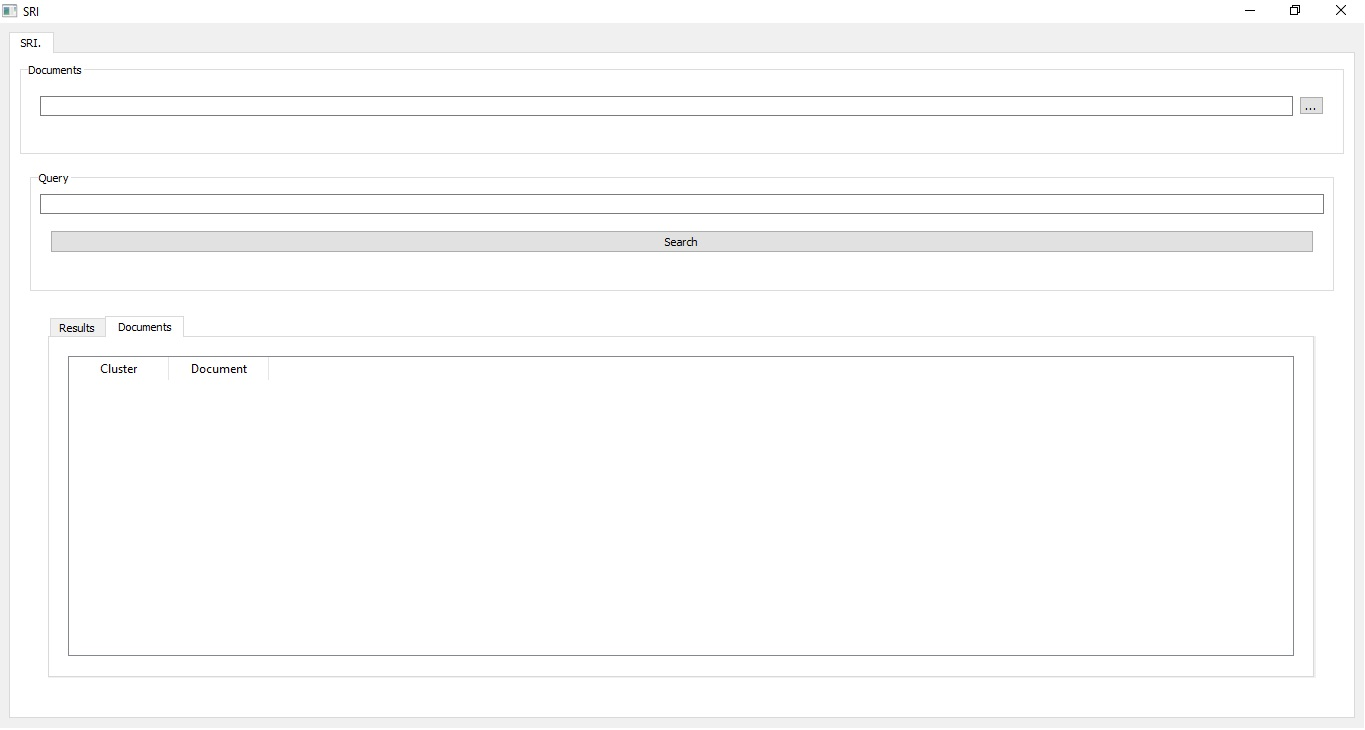
\includegraphics[width = 10cm, height = 7cm]{app/inicializando.jpg}
	\caption{}
\end{figure}

Si se da clic en los 3 puntos que se encuentran en la secci\'on Documents, se da la opci\'on de seleccionar la direcci\'on de la colecci\'on a procesar. Una vez seleccionada, saldr\'ia en esta secci\'on un cartel que dice ``Processing Documents'', mientras se est\'en procesando los documentos, como se muestra en la Fig. 2.\\

\begin{figure}
	\centering
	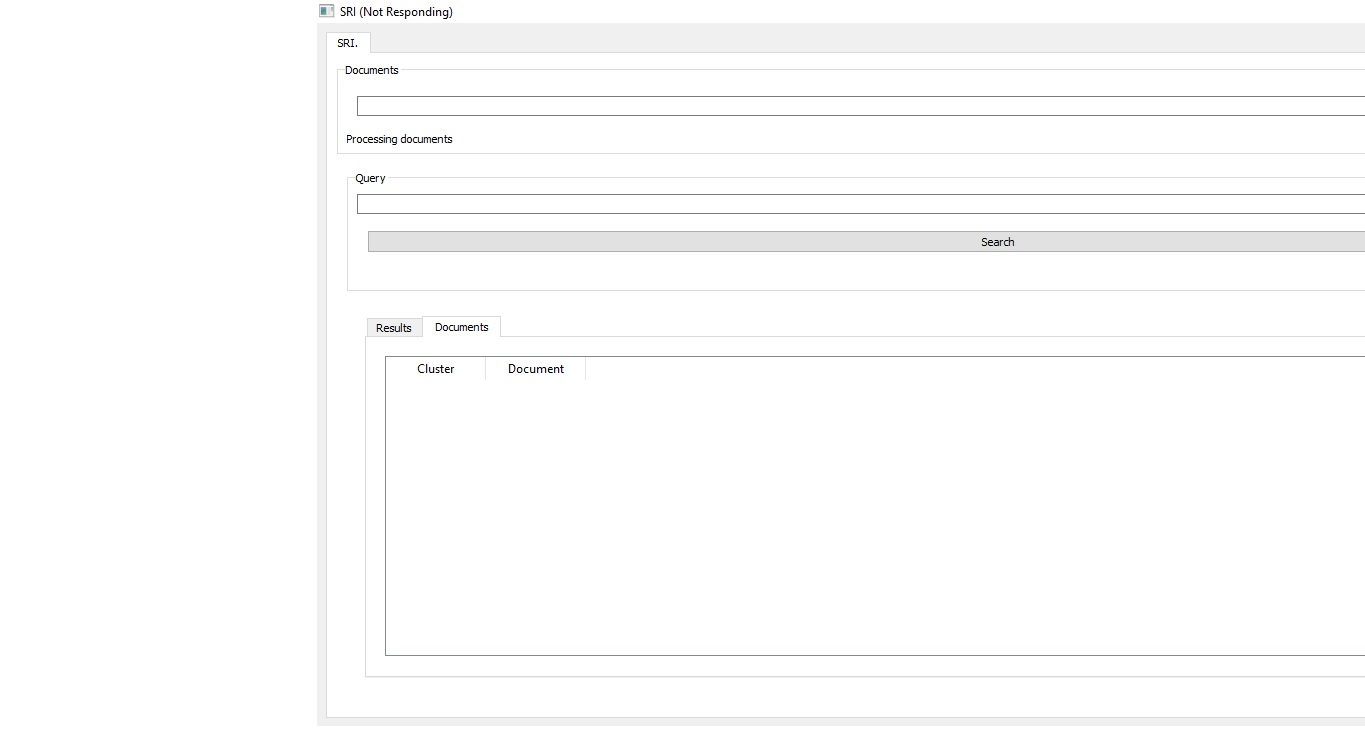
\includegraphics[width = 10cm, height = 7cm]{app/processing.jpg}
	\caption{}
\end{figure}

Una vez procesados los documentos, en la l\'inea donde se seleccion\'o la direcci\'on aparecer\'a esta, luego en el recuadro ``Documents'', en la primera columna aparecer\'a el cl\'uster al que pertenece el documento y en la segunda columna el documento . Esto se muestra en la Fig. 3.\\

\begin{figure}
	\centering
	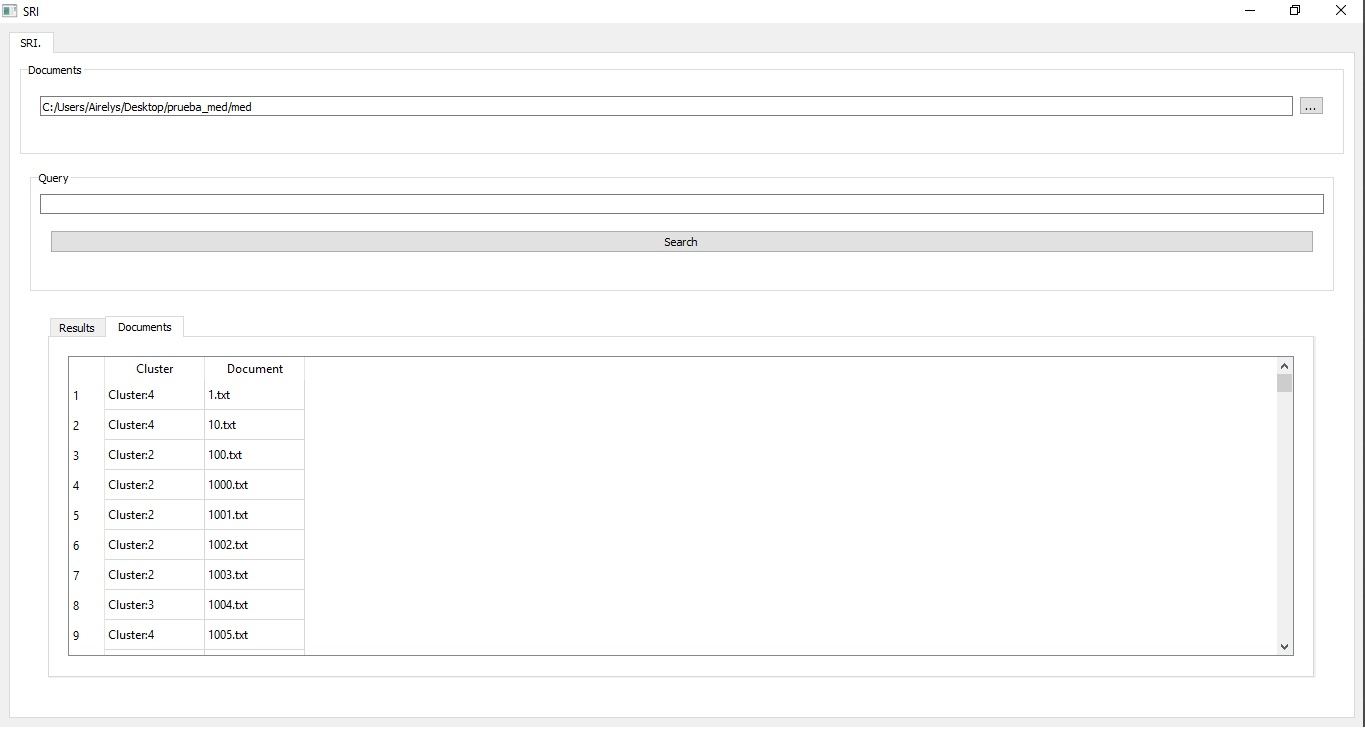
\includegraphics[width = 10cm, height = 7cm]{app/process.jpg}
	\caption{}
\end{figure}

Luego para hacer una consulta, en la secci\'on ``Query'' en la l\'inea de texto se introduce la consulta que se desea hacer y se da clic en el bot\'on ``Search''. Luego de procesar dicha consulta en la secci\'on ``Results'' se muestran los documentos que fueron recuperados, en la primera columna el cl\'uster al que pertenece el documento y en la segunda el documento. Esto se puede observar en la Fig. 4.\\

\begin{figure}
	\centering
	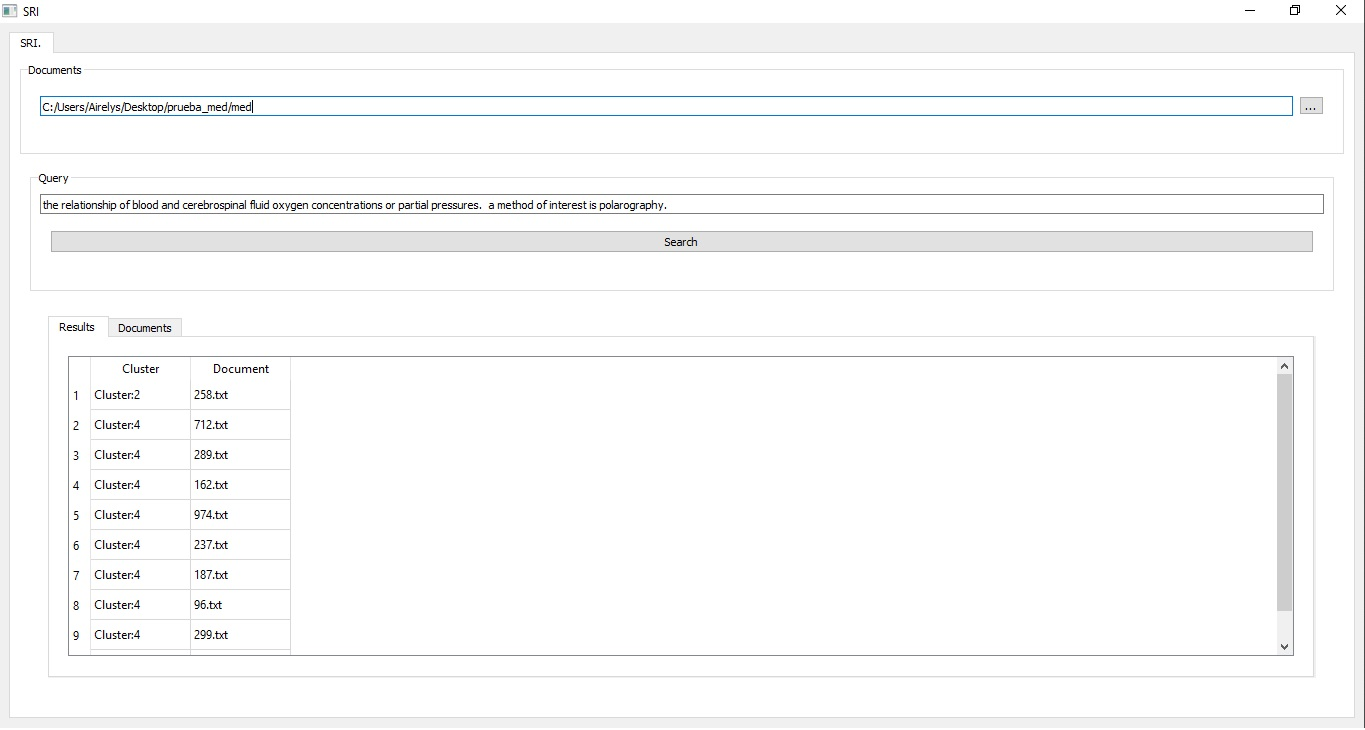
\includegraphics[width = 10cm, height = 7cm]{app/query.jpg}
	\caption{}
\end{figure}



%
\section{Evaluaci\'on del sistema}
% 

Para la evaluaci\'on del sistema se usaron las colecciones Cranfield y Medline, las cuales se dejan junto con este reporte y el c\'odigo fuente del sistema. Las colecciones se tienen en $.txt$ pues es el formato que recibe el proyecto, cada documento de la colecci\'on est\'a en un $.txt$ distinto. Las colecciones no est\'an cargadas para que se vea el procesamiento de documentos, el cual se demora un poco, pues son algo extensas las colecciones.\\

\subsection{Medidas usadas}

Para evaluar el sistema se implementaron un conjunto de medidas que los eval\'ua de acuerdo a los documentos que recupera y a los que no. La implementaci\'on de estas medidas se encuentra en \texttt{evaluation\_measures.py} y la aplicaci\'on de estas se encuentra en \texttt{evaluation.py}.\\

Antes de continuar es importante conocer algunos conjuntos:\\

\begin{list}{-}{•}
\item \textbf{REL} conjunto de documentos relevantes
\item \textbf{REC} conjunto de documentos recuperados
\item \textbf{RR} conjunto de documentos relevantes recuperados
\item \textbf{NN} conjunto de documentos no relevantes no recuperados
\item \textbf{RI} conjunto de documentos recuperados irrelevantes
\item \textbf{NR} conjunto de documentos no recuperados relevantes
\end{list}

\textbf{Precisi\'on:} eval\'ua la consulta de acuerdo a los documentos relevantes que se recuperan.[2]\\

\begin{equation}
	P = \frac{|RR|}{|RR \cup RI|} = \frac{|RR|}{|REC|}
\end{equation}

Despu\'es de tener los documentos que fueron recuperados en la consulta, se buscan cu\'ales son relevantes con ayuda de la informaci\'on brindada por la colecci\'on, y teniendo esto, se aplica la f\'ormula. Este proceso se realiz\'o para cada consulta de la colecci\'on y los resultados obtenidos fueron promediados.\\

\textbf{Recobrado:} fracci\'on de los documentos relevantes que fueron recuperados.[2]\\

\begin{equation}
	R = \frac{|RR|}{|RR \cup NR|} = \frac{|RR|}{|REL|}
\end{equation}
 
Con ayuda de la informaci\'on que brinda la colecci\'on se buscan los documentos relevantes para la consulta, teniendo ya los documentos recuperados se va analizando de estos cu\'ales son relevantes e igualmente se aplica la f\'ormula. El proceso se realiza para cada consulta de la colecci\'on y los resultados obtenidos se promedian.\\

\textbf{Medida F:} enfatiza la precisi\'on sobre el recobrado o viceversa.[2]\\

\begin{equation}
	F = \frac{(1 + \beta^2)PR}{\beta^2P + R}
\end{equation}

$\beta = 1$: mismo peso para la precisi\'on y recobrado
$\beta > 1$: mayor peso para la precisi\'on
$\beta < 1$: mayor peso para el recobrado

Para calcularla se usaron las dos medidas anteriores y se aplic\'o la f\'ormula. Igualmente, el proceso se realiza para cada consulta de la colecci\'on y los resultados obtenidos se promedian.\\

\textbf{Medida $F_1$:} armoniza precisi\'on y recobrado teniendo en cuenta a ambos.[2]\\

\begin{equation}
	F_1 = \frac{2PR}{P + R}
\end{equation}
 
Para su c\'alculo se us\'o el c\'alculo de la precisi\'on y el recobrado y se aplic\'o la f\'ormula. Igualmente, el proceso se realiza para cada consulta de la colecci\'on y los resultados obtenidos se promedian.\\

\textbf{R-Precisi\'on:} es el ranking de documentos relevantes a una consulta para la cual existen R documentos relevantes.[2]\\

\begin{equation}
	P_R = \frac{|RR|_R}{|RR \cup RI|_R} = \frac{|RR|_R}{|REC|_R}
\end{equation}\

Para su c\'alculo se seleccionaron los primeros R documentos recuperados y de estos se vieron cu\'ales son relevantes, de acuerdo a la informaci\'on que brinda la colecci\'on y se aplica la f\'ormula. El proceso se realiza para cada consulta de la colecci\'on y los resultados obtenidos se promedian.\\

\textbf{Proporci\'on de fallo:} tiene en cuenta la cantidad de documentos irrelevantes y el ranking.[2]\\

\begin{equation}
	Fallout = \frac{|RI|}{|RI \cup NI|} = \frac{|RI|}{|I|}
\end{equation}

Con la diferencia de los documentos recuperados y de los recuperados relevantes, se tiene el conjunto de los documentos recuperados irrelevantes; con la diferencia del total de documentos y los documentos relevantes se tiene el conjunto de los documentos irrelevantes; luego, se aplica la f\'ormula y se repite el proceso para cada consulta de la colecci\'on y los resultados se promedian.\\

\subsection{An\'alisis de los resultados}

Los an\'alisis de los resultados se encuentran en t\textbf{evaluation.py} donde en la l\'inea 8 se especifica la direcci\'on de la colecci\'on de los documentos, en la l\'inea 18 el documento con las consultas a realizar, en la l\'inea 45 la direcci\'on del archivo con las relaciones de relevancia y en la l\'inea 12 el umbral de similitud.\\

Para el an\'alisis de los resultados se utiliz\'o la colecci\'on Cranfield que cuenta con 1400 documentos y 225 consultas.[4]\\

Resultados promedios para un umbral de similitud de 0.09:\\
\begin{list}{-}{•}
\item Precisi\'on: 0.10901124131401935
\item Recobrado: 0.6467905483092768
\item Medida F $\beta = 0$: 0.10901124131401935
\item Medida $F_1$: 0.1694418791771936
\item Medida F $\beta = 2$: 0.27972846259960443
\item $R-precision_10$: 0.25644444444444453
\item Proporci\'on de fallo: 0.038643443412114016
\end{list}

Se observa que el recobrado promedio es alto, un resultado bueno para esta medida, sin embargo, la precisi\'on es bastante baja, aunque la $R-precision_10$ es un poco m\'as alta que la \'ultima. La proporci\'on de fallo tiene un bajo valor.\\ 

Resultados promedios para un umbral de similitud de 0.13:\\
\begin{list}{-}{•}
\item Precisi\'on: 0.08264034598980041
\item Recobrado: 0.17700588420630056
\item Medida F $\beta = 0$: 0.08264034598980041
\item Medida $F_1$: 0.09549277220095578
\item Medida F $\beta = 2$: 0.12221300248442155
\item $R-precision_10$: 0.0853333333333333
\item Proporci\'on de fallo: 0.012351378630590288
\end{list}

Con un umbral de similitud de 0.13 se observa que disminuy\'o considerablemente tanto la precisi\'on como el recobrado. Los resultados son malos para este umbral.\\

Resultados promedios para un umbral de similitud de 0.11:\\
\begin{list}{-}{•}
\item Precisi\'on: 0.2008825095059054
\item Recobrado: 0.5171964188598902
\item Medida F $\beta = 0$: 0.2008825095059054
\item Medida $F_1$: 0.24577953319539336
\item Medida F $\beta = 2$: 0.3341486091074317
\item $R-precision_10$: 0.25377777777777794
\item Proporci\'on de fallo: 0.015071520080302098
\end{list}

Si se fija el umbral de similitud en 0.11 se observa un recobrado bueno, la precisi\'on, aunque es un poco baja a\'un , es la m\'as alta obtenida. Los mejores valores para la Medida F y la Medida $F_1$ son los obtenidos con este umbral.\\


Para el an\'alisis de los resultados tambi\'en se utiliz\'o la colecci\'on Medline que cuenta con 1033 documentos y 30 consultas.[4]\\


Resultados promedios para un umbral de similitud de 0.12:\\
\begin{list}{-}{•}
\item Precisi\'on: 0.5360821109288602
\item Recobrado: 0.3127791713751234
\item Medida F $\beta = 0$: 0.5360821109288602
\item Medida $F_1$: 0.361086724788996
\item Medida F $\beta = 2$: 0.32718245210365
\item $R-precision_10$: 0.4433333333333333
\item Proporci\'on de fallo: 0.0037987334206573643
\end{list}

En este caso, la precisi\'on es alta, sin embargo el recobrado es un poco bajo, aunque la $R-precision_10$ es buena. La proporci\'on de fallo es peque\~na.\\

Resultados promedios para un umbral de similitud de 0.1:\\
\begin{list}{-}{•}
\item Precisi\'on: 0.5700169377692599
\item Recobrado: 0.43652582642712573
\item Medida F $\beta = 0$: 0.5700169377692599
\item Medida $F_1$: 0.4501325525357391
\item Medida F $\beta = 2$: 0.43590182433222535
\item $R-precision_10$: 0.56
\item Proporci\'on de fallo: 0.0053463336700038805
\end{list}

Ahora, se observa una mejor\'ia en el recobrado y la precisi\'on sigue buena, la $R-precision_10$ tambi\'en aument\'o.\\

Resultados promedios para un umbral de similitud de 0.09:\\
\begin{list}{-}{•}
\item Precisi\'on: 0.5359934670090849
\item Recobrado: 0.5021524639279512
\item Medida F $\beta = 0$: 0.5359934670090849
\item Medida $F_1$: 0.47893542575549086
\item Medida F $\beta = 2$: 0.4853989717474617
\item $R-precision_10$: 0.6000000000000001
\item Proporci\'on de fallo: 0.007766367574079214
\end{list}

Si se fija el umbral de similitud de 0.09 se observa una compensaci\'on de la precisi\'on y recobrado, donde la Medida F con $\beta = 0$ y $\beta = 2$ y la Medida $F_1$ la manifiestan. La $R-precision_10$ es muy buena.\\


 
%
\section{Ventajas y desventajas del sistema desarrollado}
% 

El proyecto desarrollado indica ser aceptable, pues como se vio en la secci\'on anterior da respuestas bastante buenas. Las m\'etricas que se usan para evaluar los sistemas de recuperaci\'on de informaci\'on dieron buenos resultados. Se tiene implementada una forma de expansi\'on de consulta y un algoritmo de clustering. Se tiene una interfaz visual que es amigable para el usuario. Adem\'as, si se desea a\~nadir alguna nueva funcionalidad no se pasar\'ia mucho trabajo porque est\'a hecho y pensado para que futuros autores puedan trabajar en \'el f\'acilmente.\\
\\
Aunque el sitema da buenos resultados, la parte de procesar los documentos se demora un poco, sobre todo para colecciones muy grandes y con documentos extensos. Otra desventaja es que solo lee documentos en formato $.txt$. Adem\'as, el sistema solo puede ser usado localmente, no en la web.\\

%
\section{Recomendaciones y Conclusiones}
% 

Adem\'as de las t\'ecnicas utilizadas en este proyecto se considera que pueden a\~nadirse otras que mejoren mucho m\'as la propuesta. Primeramente, el m\'etodo de leer documentos se puede ampliar m\'as para que se lean otros formatos como $.pdf$, $.docx$, $.html$, etc; pues el de este proyecto solo lee $.txt$. Tambi\'en puede proponerse alg\'un mecanismo de optimizaci\'on para que se realice un poco m\'as r\'apido el procesamiento de documentos, pues como ya se mencion\'o se demora un poco en procesarlos. Se pueden a\~nadir otras formas de expandir las consultas como los tesauros. Adem\'as, se puede a\~nadir crawling como forma de recuperaci\'on en la web.\\
\\
Siempre los proyectos se pueden mejorar un poco m\'as, siempre queda algo por hacer que lo mejore.\\
\\
Desarrollar un Sistema de Recuperaci\'on de informaci\'on es algo trabajoso y que lleva estudio. Hay que intentar responderle al usuario de la mejor manera posible, o sea, se deben satisfacer sus peticiones. Cada desici\'on que se tome es pensando si dar\'a mejores resultados. Son varias fases por las que hay que pasar para mostrar buenas respuestas y siempre intentando hacer un poquito m\'as.\\


%
\section{Referencias}
%


[1]. Tolosa y Bordignon(2007)\\

[2] Conferencias de Sistemas de Recuperaci\'on de Informaci\'on.\\

[3] Primeros pasos en PyQt5 y QtDesigner: Programas gr\'aficos con python. (medium.com)\\

[4] http://ir.dcs.gla.ac.uk/resources/test\_collections/



\end{document}
